\documentclass[../report.tex]{subfiles}

\begin{document}

% Chapter State of the art
% - Concepts (before diving into the protocoles, it is important to understand some concepts)
% - Outlines of the KAPE landscape (all PAKEs, history, overview)
% - Mains PAKEs (differences, improvement, tableau comparatif, pas besoin de décrire les constructions)
%   - EKE
%   - SRP
%   - OPAQUE
%   - KHAPE
% - PAKE choice (and reasons)

% (Attack on PAKEs ?)


% Chapter OPAQUE or Chapter KHAPE (depending on the PAKE choice)
% - detail construction (protocol) of the choosen PAKE

\chapter{State of the art}

\section{Notation}

\section{History of PAKEs}
\paragraph{EKE (1992)}
\paragraph{EKE variants (PAK, PPK, PAK-X)}
\paragraph{OKE}
\paragraph{SNAPI}
\paragraph{PEKEP}
\subsection{Symmetric PAKE}
\subsection{Asymmetric PAKE}
\paragraph{SRP (1998)}
\paragraph{OPAQUE (2018)}
\paragraph{KHAPE (2021)}





\section{Main PAKEs}


\subsection{\writingFormulationClean{EKE}}
\paragraph{\writingFormulationClean{Introduction}}

EKE (for Encrypted Key Exchange) was proposed in 1992 by Bellovin and Merritt \cite{EKE_Paper} and is the first PAKE protocol. 
It allows two parties that share a common password to exchange information over an insecure channel.
It is a simple protocol that is designed to prevent offline dictionary attacks on the password.
It uses a combination of asymmetric and symmetric cryptography.
The asymmetric keys are ephemeral and are exchanged between the client and the server by encrypting it with the shared symmetric key --- which is derived from the password.
This allows securing the exchange against Man-in-the-Middle attack. % more ?
However, this protocol requires that both party share a secret --- namely the password. This means that the server has to store and process the password in cleartext which is strongly discouraged. % details ?


Multiple cryptographic primitive can be used for the asymmetric part such as RSA, ElGamal or DH but the majority of EKE variants use DH \cite{Breaking_EKE}. % more ? why ?

Overall, EKE got broken and therefore should not be used. % TODO source. all EKE ? EKE-DH also ?


\paragraph{\writingFormulationClean{Construction}}

\begin{figure}[h]
 \centering
 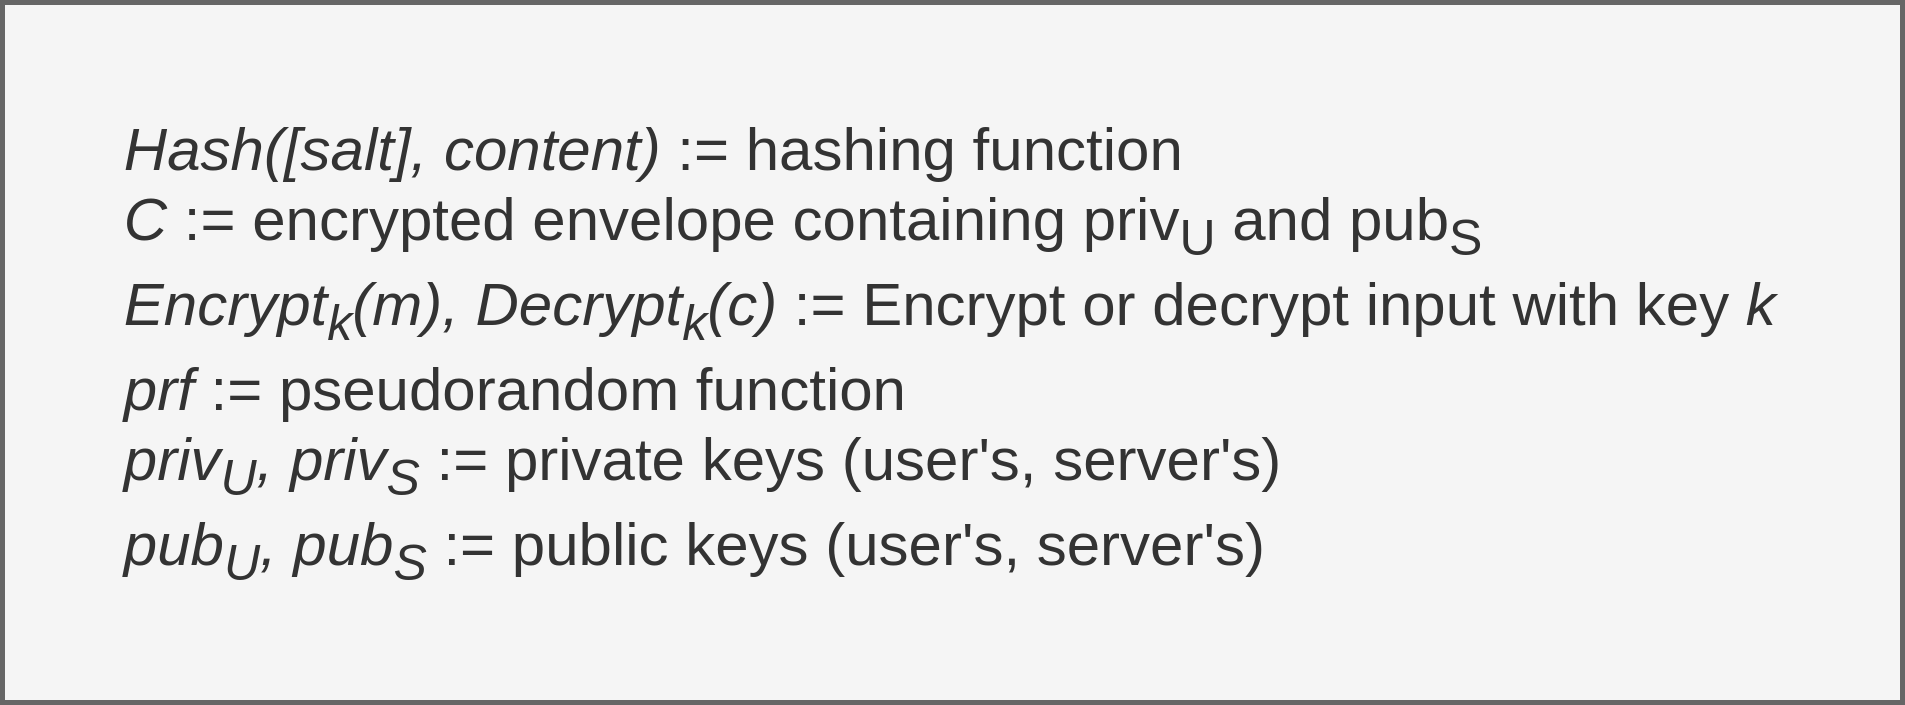
\includegraphics[width=10cm]{notation.png}
 \caption{Schema notation.}
 \label{fig:notation}
\end{figure}



\begin{figure}[h]
 \centering

 \setlength{\fboxsep}{10pt}
 \setlength{\fboxrule}{1pt}
 \fbox{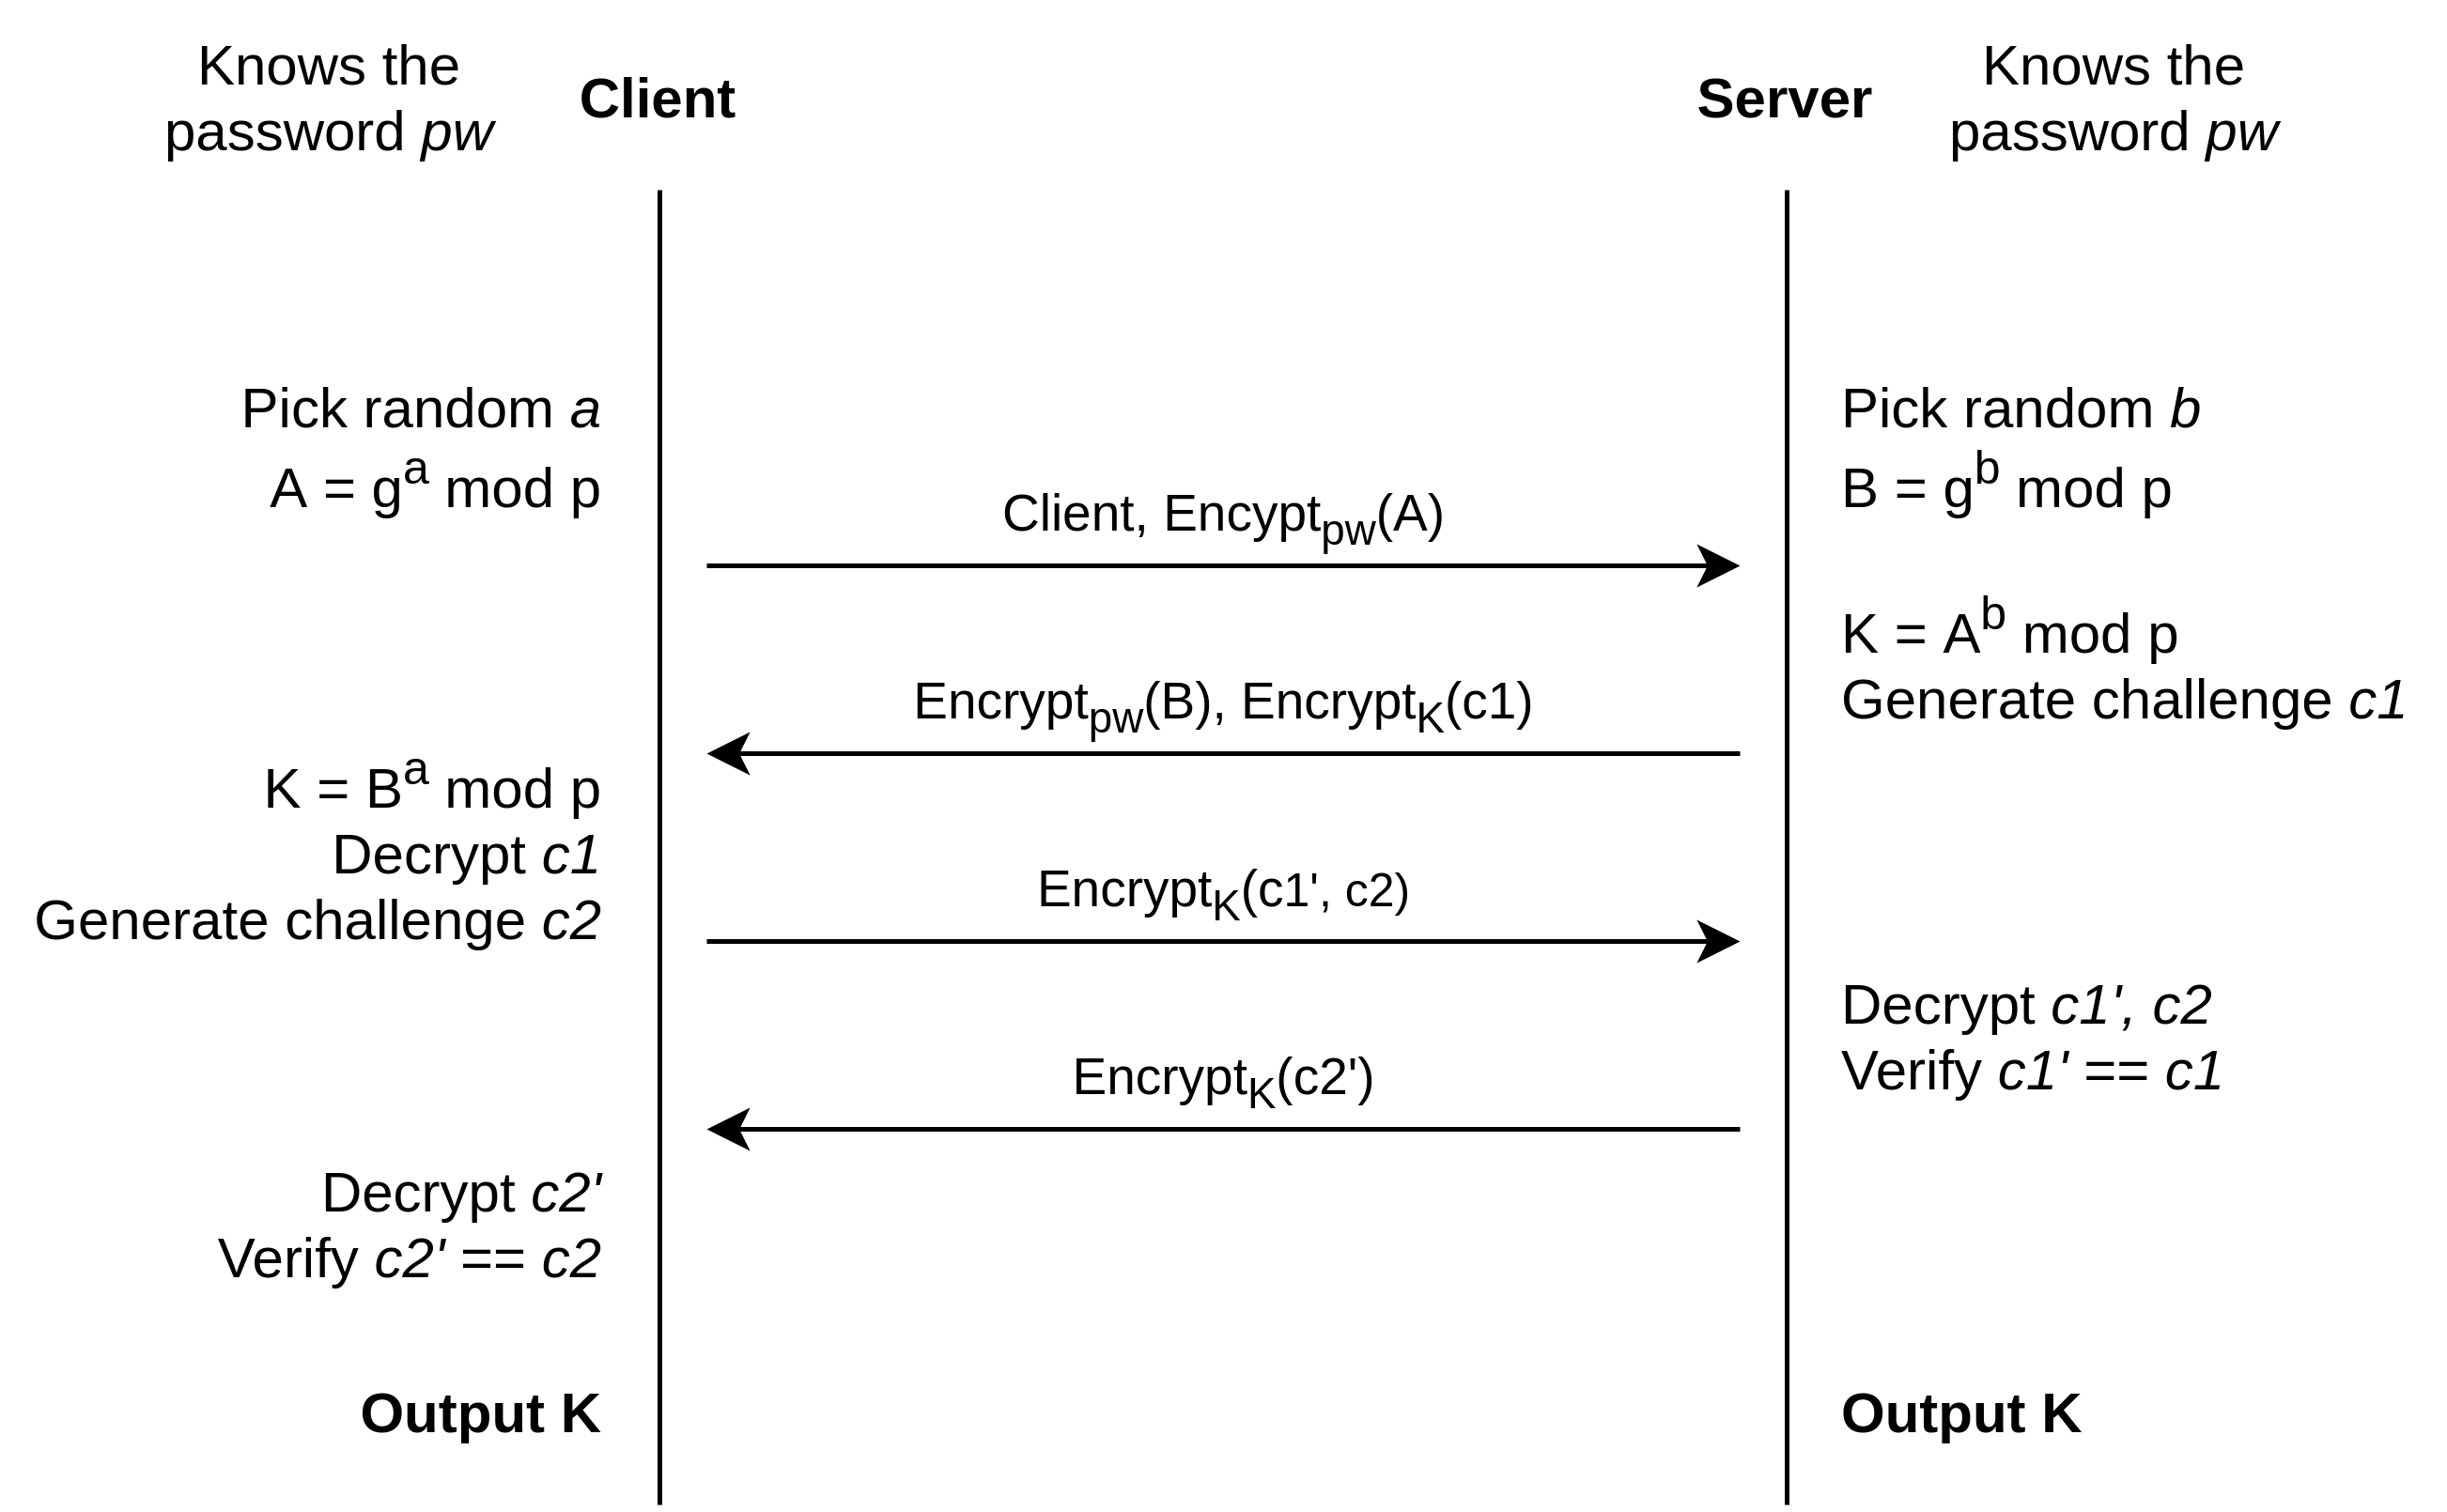
\includegraphics[width=\textwidth-22pt]{EKE.png}}

 \caption{Login process with EKE (EKE-DH) protocol. (See Fig. \ref{fig:notation} for notations)}
 \label{fig:EKE_DH}
\end{figure}

The figure \ref{fig:EKE_DH} shows the EKE protocol --- built with DH ---  during login process.
The steps are the following :

\begin{enumerate}
 \item Like a standard DH exchange, both client and server pick a random secret value $a$ and $b$.
 \item Client computes $A$, encrypt it using the password and send the result to the server in addition to it identifies (e.g., username).
 \item Server decrypts ciphertext using the password to obtain $A$. He computes $B$ and $K$. He encrypts $B$ using the password and encrypt a randomly generated challenge $c1$ using $K$. He sends the resulting ciphertext to the client.
 \item The client decrypts $B$ using the password and compute $K$. He decrypts $c1$ with $K$ and also generate a random challenge $c2$. He concatenate the two challenges, encrypt them using $K$ and send the result to the server.
 \item Server decrypt the ciphertext and check that both sent and received $c1$ match. If it's the case, the server is assured that the client possesses the same password. The server has authenticated the client. He finishes by encrypting $c2$ and sending the result.
 \item Client decrypts the ciphertext and check that both sent and received $c2$ match. If it's the case, the client is assured that the server possesses the same password and therefore is authenticated. The client has authenticated the server.
\end{enumerate}


%%% Login ?

\paragraph{\writingFormulationClean{Register}}
The protocol doesn't mention registration. It is assumed that both parties already share a common secret, the password. A secure channel is therefore necessary to share the password in the first place.


% ====================================================================================



\subsection{\writingNotes{SRP}}
SRP (for Secure Remote Password), 1998.




% ====================================================================================



\subsection{\writingFormulationClean{OPAQUE}}


\paragraph{\writingFormulationClean{Design}}
Jarecki and al. \cite{OPAQUE_Paper}. introduce the definition of Strong aPAKE (SaPAKE): an aPAKE secure against pre-computation attacks.

They provide two modular constructions, called the OPAQUE protocol that allow building SaPAKE protocols. The first construction allows enhancing any aPAKE to a SaPAKE while the second allows enhancing any Authenticated Key-Exchange (AKE) protocol (that are secure against KCI attacks) to a SaPAKE.
The security of these two construction is based on Oblivious PRF (OPRF) functions. % cite ?

These functions allow for each party, namely the client and the server, to input a secret value and then the client can use the output as a key. Neither party can learn the other party's secret, and the server cannot learn the output of the function.

Overall, the OPAQUE protocol allows to secure authentication from the simplest applications to the most sensitive ones.


%%% Implementation ? HMQV ?


% \paragraph{\writingNotes{Additional features}}
% 
% In addition to providing a Strong aPAKE protocol, OPRF provides other interesting security features that can be used with OPAQUE.
% 
% 
% "Supports user-side password hardening"
% "has a built-in facility for password-based storage-and-retrieval of secrets and credentials"
% "accommodates a user-transparent server-side threshold implementation"
% "far more secure alternative to the practice of deriving low-entropy secrets directly from a user's password"


\paragraph{\writingFormulationClean{Construction}}

\begin{figure}[h]
 \centering

 \setlength{\fboxsep}{10pt}
 \setlength{\fboxrule}{1pt}
 \fbox{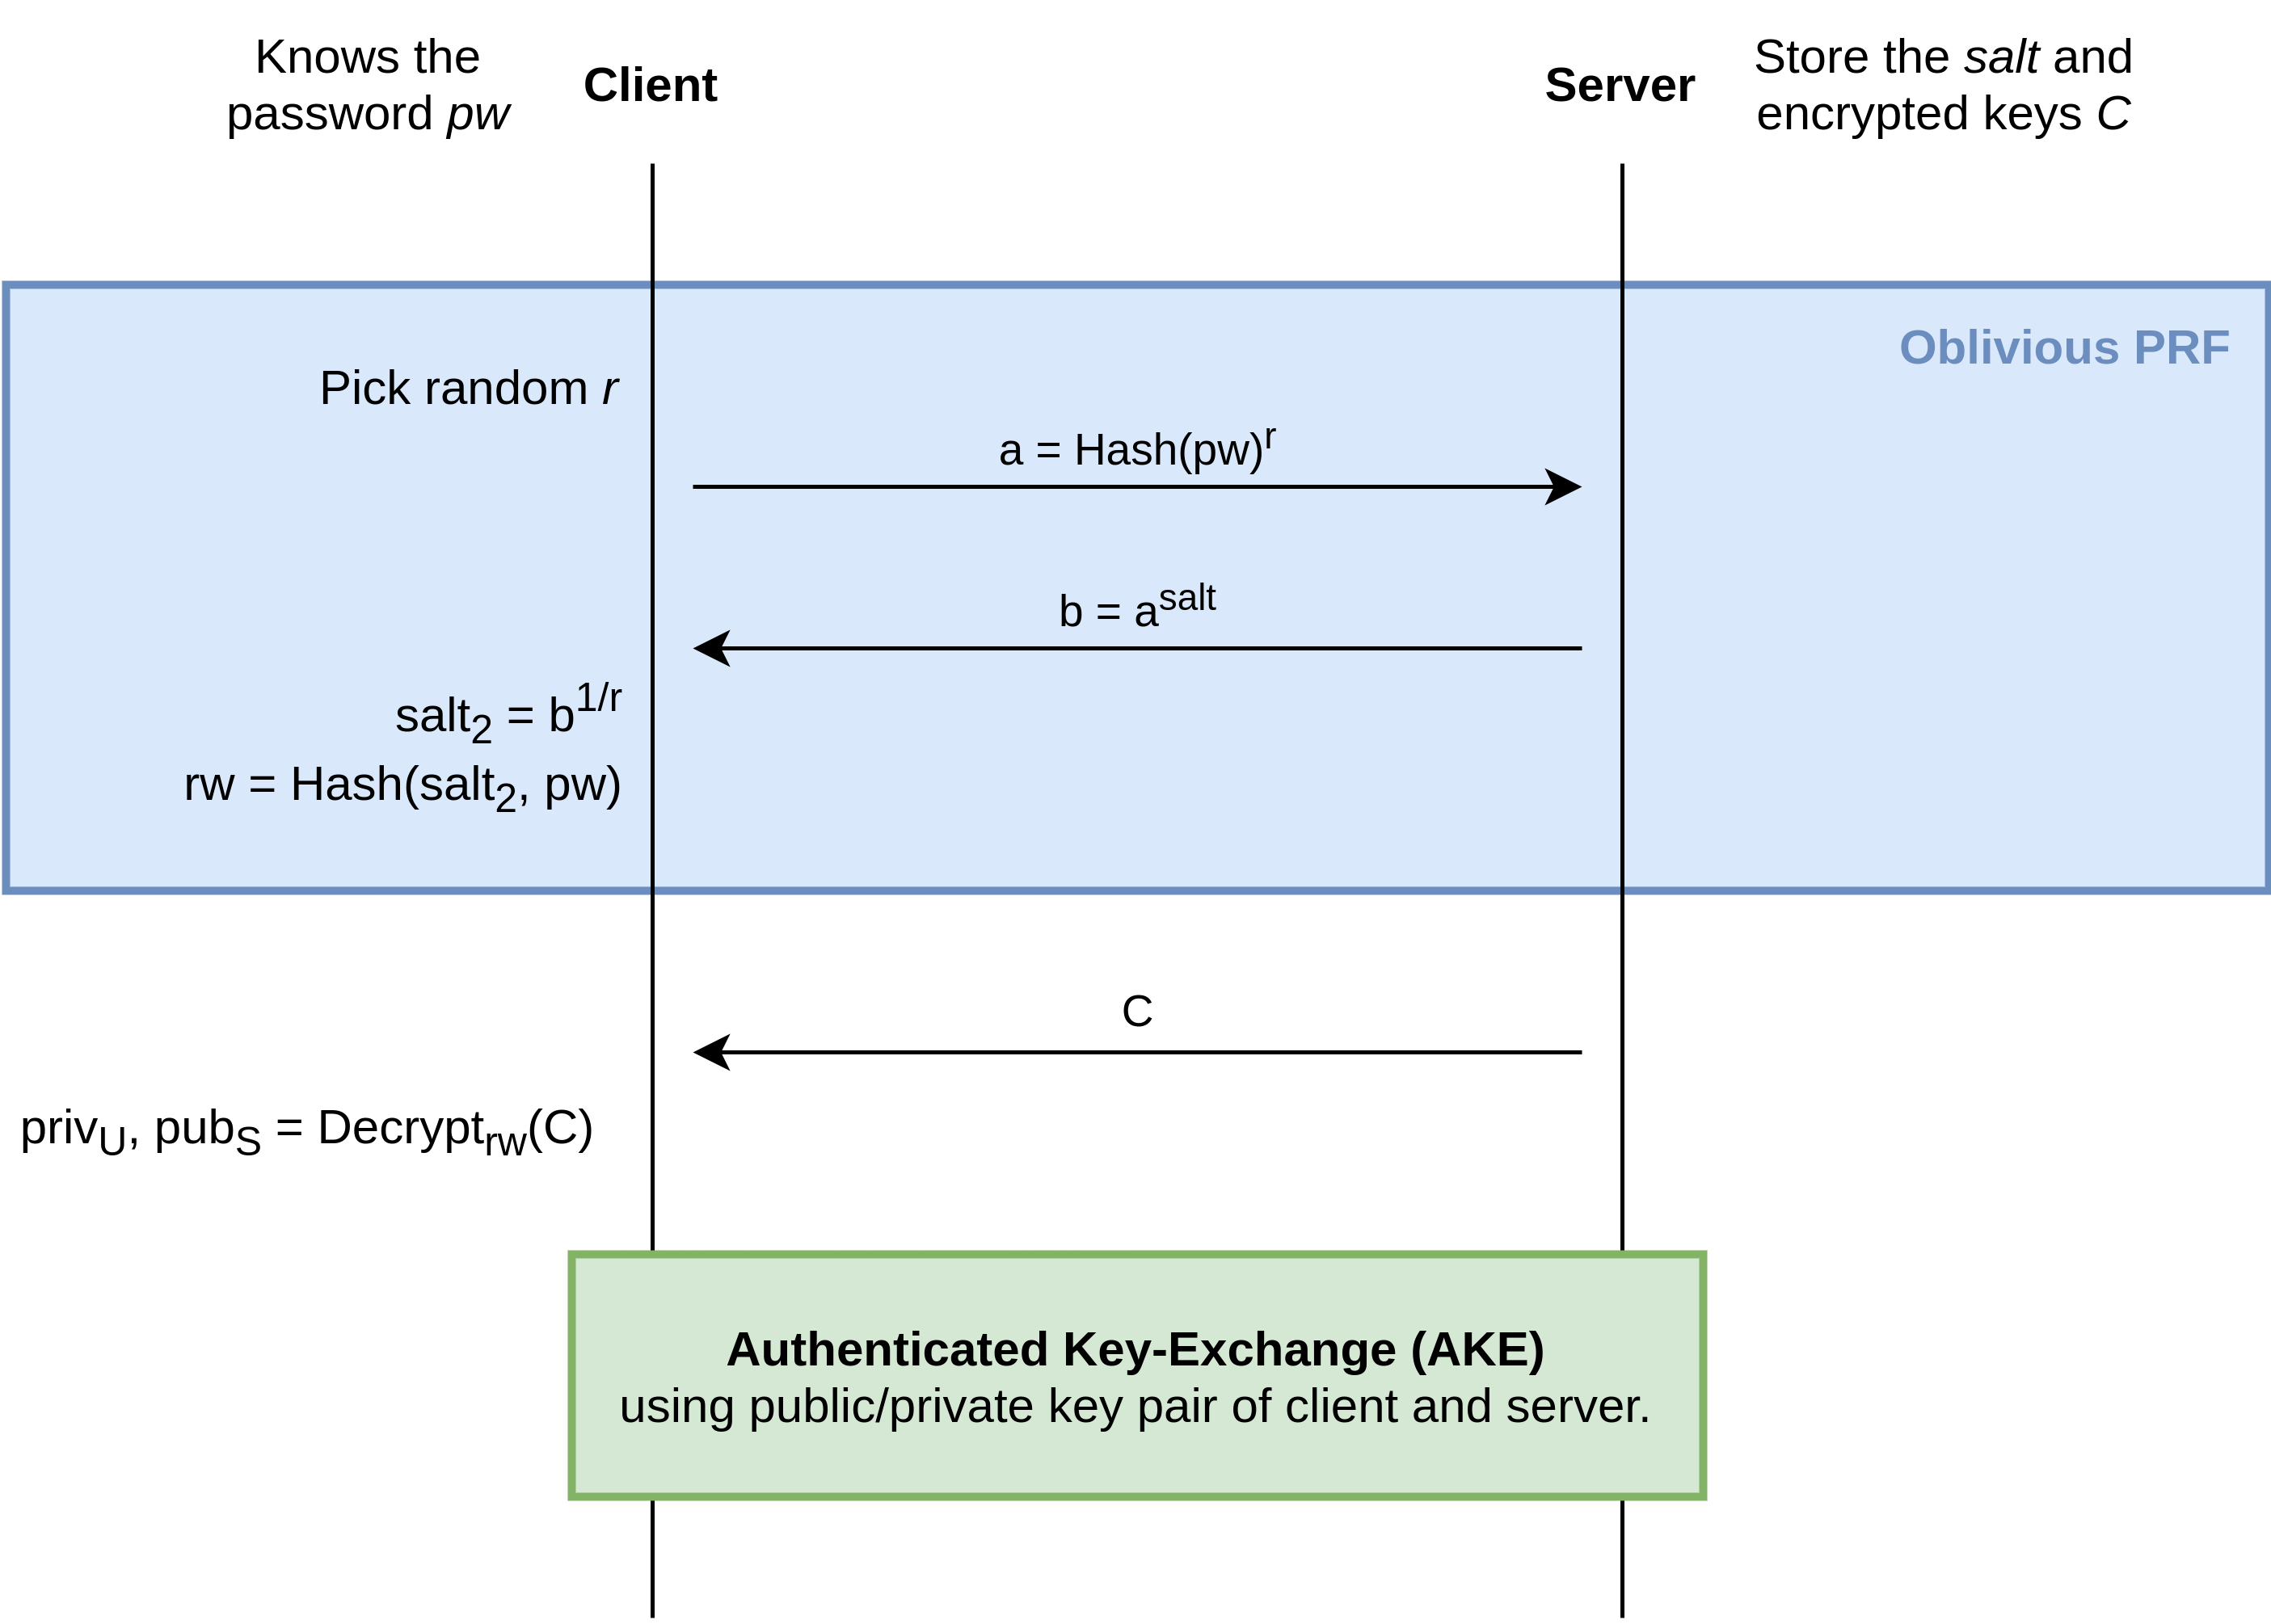
\includegraphics[width=\textwidth-22pt]{OPAQUE.png}}

 \caption{Login process with generic OPAQUE (OPRF-AKE) protocol. (See Fig. \ref{fig:notation} for notations)}
 \label{fig:OPAQUE_AKE}
\end{figure}

The figure \ref{fig:OPAQUE_AKE} shows the OPAQUE protocol --- built with OPRF and AKE --- during login process.
The steps are the following :


\begin{enumerate}
 \item Generate a random value $r$ to blind the hash of passwords so that the server cannot retrieve the password from the mapping.
 \item Send result to the server.
 \item Server add the salt to the password.
 \item The client calculates the exponent of the inverse of $r$ to de-blind the value. He cannot retrieve salt.
 \item With the secret salt $salt_2$, client compute secret key $sk$.
 \item Server send encrypted keys $C$ to clients. $C$ contains server's public key and client's private key encrypted with $rw$.
 \item If the password entered is correct, client uses $rw$ to decrypt $C$ and retrieve his private key $priv_U$.
 \item With both keys, client and server run an authenticated key exchange for mutual authentication.
\end{enumerate}


\paragraph{\writingFormulationClean{Register}} \label{sec:opaque_register}
The client registration is the only part of the protocol that requires a secure channel where both parties can authenticate each other.


The protocol is proposed with a server-side registration where the client sends his password through the secure channel. The server generates a salt and computes OPRF function with the client's password and salt. Server also generates two private keys (one for the client and one for the server) and their corresponding public key. He encrypts client's private key and server's public key with OPRF output as a key and store the ciphertext.


This method is not ideal as it requires that the user send its cleartext password to the server making it vulnerable to miss-handling or server-side vulnerabilities discussed in the introduction.


\cite{OPAQUE_Paper} also note that ideally, one wants to implement a client-side registration where the client choose a password and the server choose a secret salt and input them in the OPRF function. The client generates a public/private key pair, and the server do the same. Server sends his public key to the client. Client encrypts his private key and server's public key using OPRF output as a key. He then sends the ciphertext to the server with his public key.
This way, the server never see the cleartext password, the OPRF output and the client's private key. This is a major improvement in terms of security.

However, this also comes with a downside as the server is no longer able to check password rules. This operation needs to be done client side.


\paragraph{\writingFormulationClean{Login}}
For the login phase, the client enters its password in the OPRF and the server send the ciphertext to the client.
If the password entered is correct, the client can decrypt the ciphertext with OPRF output to obtain his private key and the server's public key.
He then uses these keys to run an authenticated key exchange with the server.

On the other hand, if the password is wrong, the OPRF output is totally different and the ciphertext decryption makes the keys incorrect and the server will refuse it during the key exchange. % TODO confirmation



% ====================================================================================



\subsection{\writingFormulationBrut{KHAPE}}
\paragraph{\writingFormulationBrut{Introduction}}

OPAQUE security relies entirely on the strength of the OPRF. If OPRF gets broken --- for example by cryptanalysis, quantum attacks or security compromise --- an adversary can compute an offline dictionary attack on the user's password. This is especially critical considering that there are currently no known quantum-safe OPRFs.

KHAPE (for Key-Hiding Asymmetric PakE) \cite{KHAPE_Paper} is a variant to the OPAQUE protocol. Instead of using OPRF as a main tool to archive security, it becomes an optional part of the protocol and KHAPE use two other concepts to archive security: non-committing encryption and key-hiding AKE. % TODO non-commiting encryption ??

% Like OPAQUE, in KHAPE each party has a private/public key pair that they use to compute the key exchange and the client store it's private key (and server's public key) on the server, encrypted by his password.
% Since KHAPE doesn't require a OPRF run before decrypting the ciphertext containing the client's private key, an adversary could eavsedrop an exchange between the client and the server. He can save the ciphertext and save the public key used by the client during the AKE. He can then compute an offline dictionary attack using a list of candidat password to decrypt the ciphertext until he find a match with the server's public key that he recorded sooner.
% To avoid this kind of attacks, KHAPE use 2 mains mechanisms. 1) Non-commiting encryption, 2) Key-hiding AKE.


% ``Two key ideas are: (i) dispense with authentication of the
% credentials4 and instead use a non-committing encryption where decryption of
% a given ciphertext under different keys cannot help identify which key from a
% candidate set was used to produce that ciphertext; and (ii) using a key-hiding
% AKE. The latter refers to AKE protocols that require that no adversary, not even
% active one, can identify the long-term keys used by the peers to an exchange even
% if provided with a list of candidate keys (a notion reminiscent of key anonymity
% for public key encryption [8]).'' \cite{KHAPE_Paper}


KHAPE is not a Strong aPAKE like OPAQUE. But it can be made a SaPAKE following the aPAKE to SaPAKE compiler from \cite{OPAQUE_Paper} using OPRF.

So OPRF is optional with KHAPE and just allow making it a SaPAKE. In addition, it also allows using OPRF features such as server-side threshold implementation that doesn't require any change from the client. If OPRF fails, KHAPE just loss these functionalities but the rest of the security remain in contrary to OPAQUE.


% Useful ?
In terms of implementation, \cite{KHAPE_Paper} prove that 3DH and HMQV are key-hiding AKE and can be used in KHAPE. % TODO see citation in KHAPE_Paper for 3DH and HMQV
It also shows that some KEM-based AKE like SKEME can be adapted to archive similar result if they are instantiated with a key-hiding KEM. % TODO cites 3DH, HMQV, SKEME papers


% \paragraph{\writingNotes{Mains differences with OPAQUE}}
% - KHAPE is computationally more performant than OPAQUE when the OPRF is not used and the performances become similar when OPRF is used.
% - "KHAPE seems more conducive to post-quantum security via post-quantum key-hiding KEMs."
% 
% - KHAPE allow less AKEs (no signature-based protocols such as SIGMA)
% - KHAPE use ``idea cipher model'', OPAQUE use ``random oracle model'' (stronger ?)
% 
% - with OPAQUE the client learns first if an authentication attempt is succeed or not. with KHAPE, the server learns first which make it easier to count failed attempt in case of an online password guessing attack.
% - KHAPE (without OPRF) cost is ~= same cost as KE cost where OPAQUE cost is about the double of KE cost


% Both client and server needs a public/private key pair to compute a AKE. The client encrypt it's credentials (his private key and server's public key) and store it in the server.



%%% How Key-hiding AKE works ?
%%% Ideal cipher ?



\paragraph{\writingFormulationClean{Construction}}


\begin{figure}[h]
 \centering
 
 \setlength{\fboxsep}{10pt}
 \setlength{\fboxrule}{1pt}
 \fbox{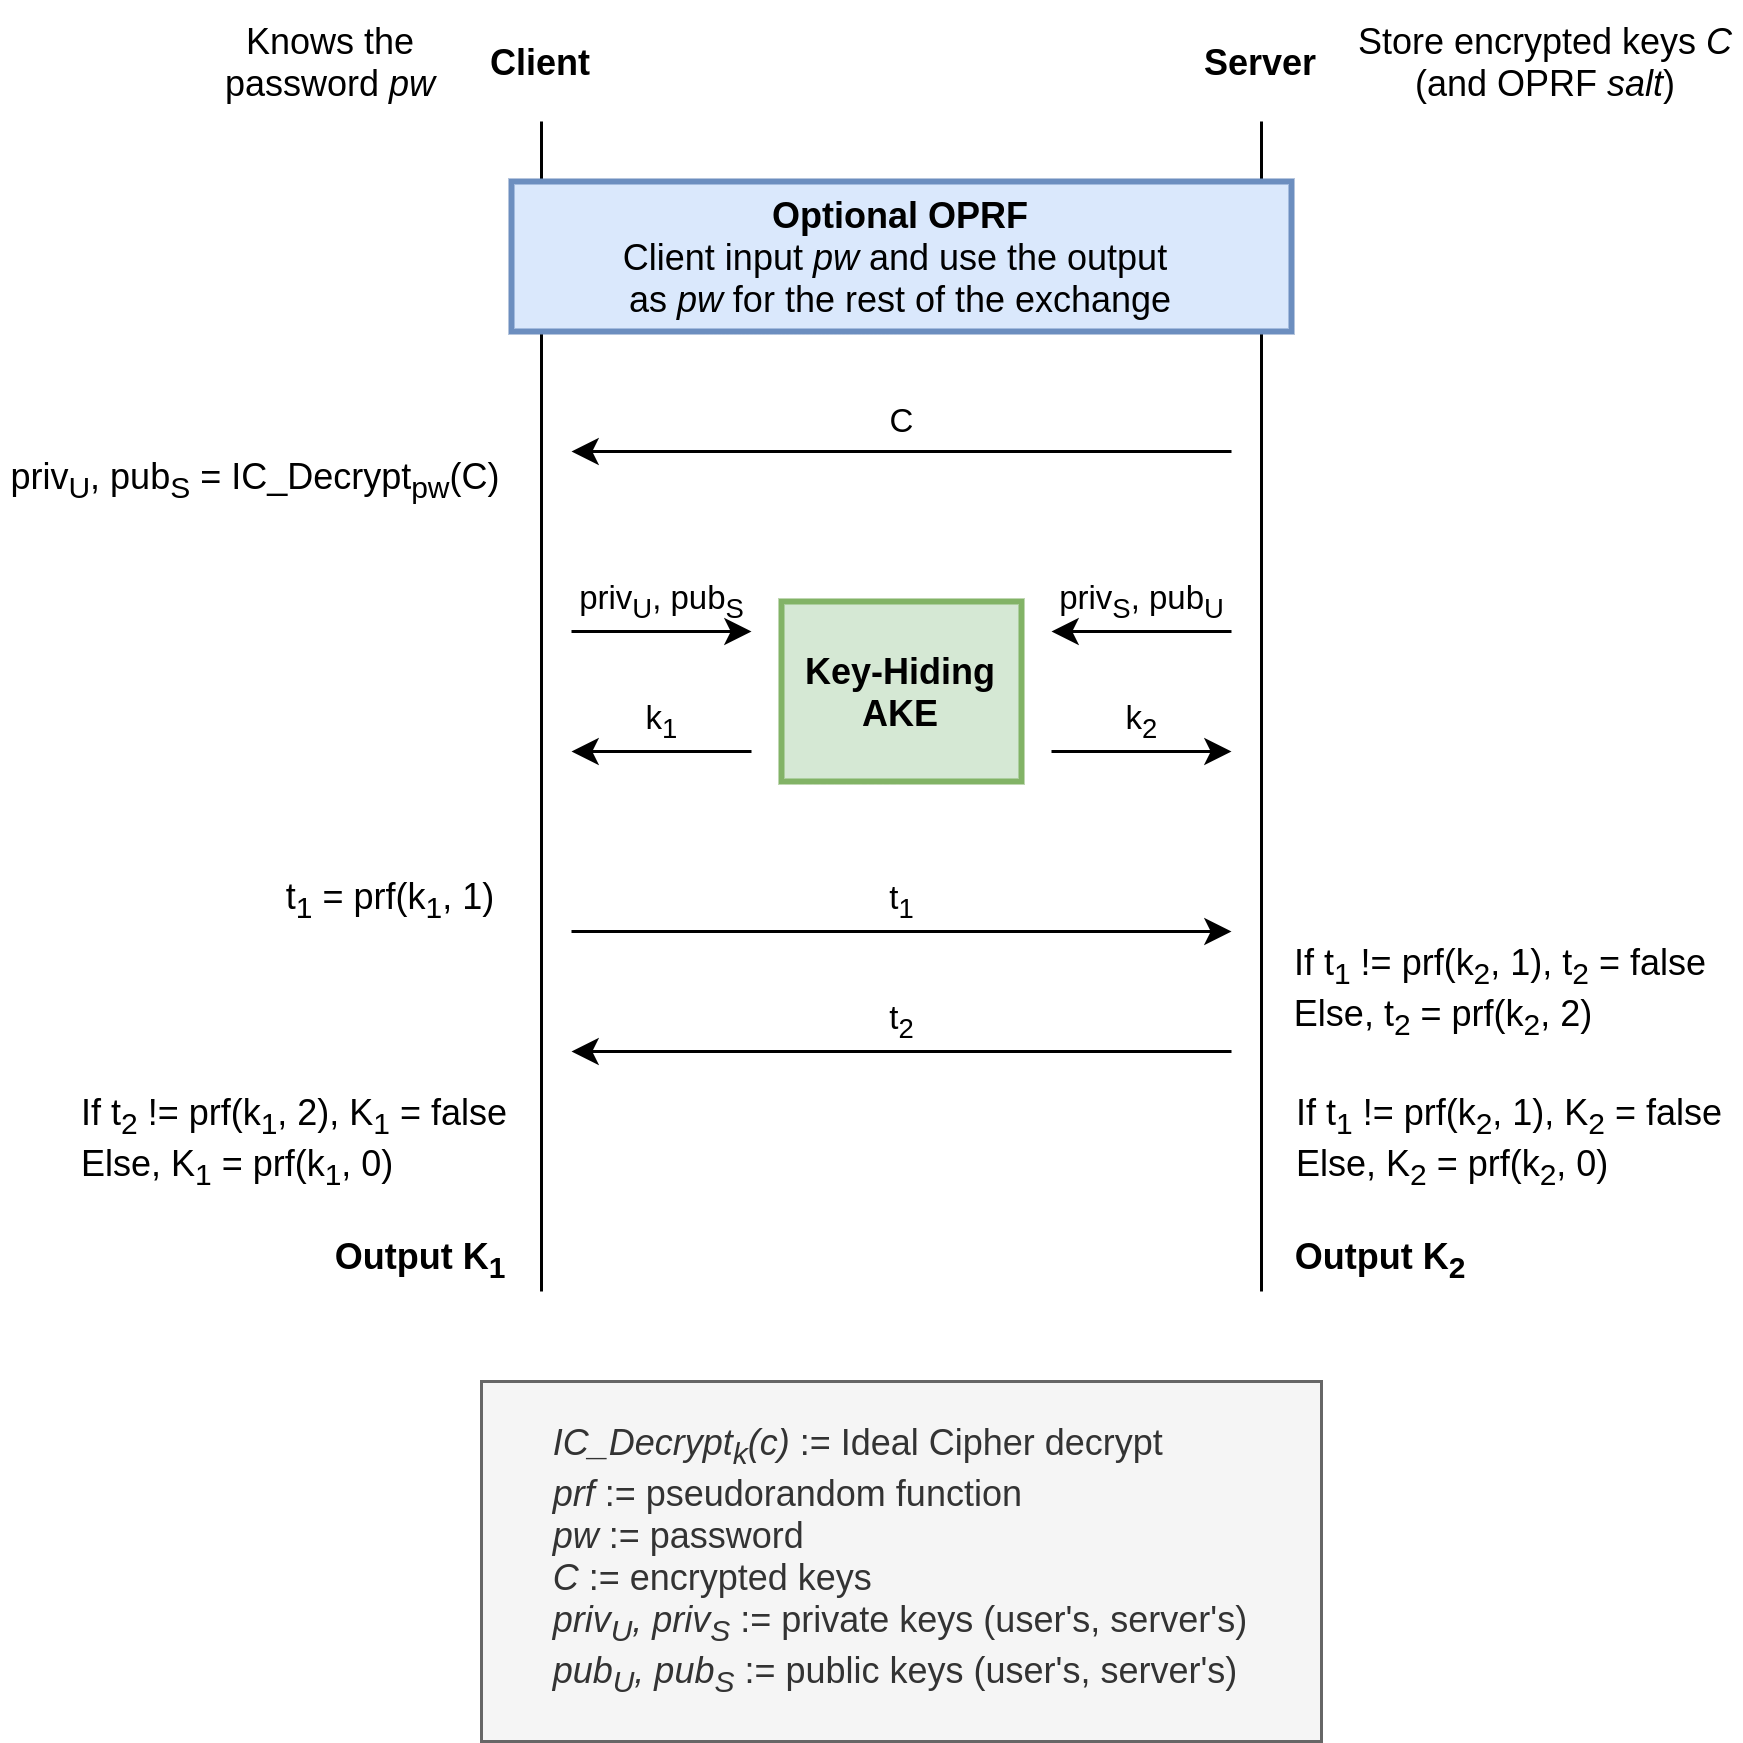
\includegraphics[width=\textwidth-22pt]{KHAPE.png}}
 
 \caption{Login process with generic KHAPE protocol. (See Fig. \ref{fig:notation} for notations)}
 \label{fig:Generic_KHAPE}
\end{figure}

Figure \ref{fig:Generic_KHAPE} shows the KHAPE protocol during login process.
The steps are the following :

\begin{enumerate}
 \item Optionally, an OPRF can be used to archive Strong aPAKE following the aPAKE to SaPAKE compiler using OPRF from \cite{OPAQUE_Paper}. The OPRF takes the client's password and server's salt as an input. Client uses the output in place of his password for the rest of the protocol.
 \item The server sends the client's encrypted envelope containing the client's private key and server's public key.
 \item The client decrypts the ciphertext using Ideal Cipher encryption schema. He uses his password or OPRF output as a key.
 \item Both parties use the public/private keys to compute a Key-Hiding Authenticated Key-Exchange.
 \item Mutual key confirmation initiated by the client.
\end{enumerate}

%%% Login and register steps
\paragraph{\writingFormulationBrut{Login}}

When the client wants to login, the server sends its encrypted credentials and the client use its password to decrypt the credentials (with or without OPRF depending on the implementation). Then he can use his credentials to compute a Key-Hiding AKE with the server.
Both party finish with a mutual key confirmation initiated by the client.


\paragraph{\writingFormulationBrut{Register}}
KHAPE has the same problem that is addressed in \ref{sec:opaque_register}.
The protocol proposes a server-side register which is less than ideal because the server can see the client’s password and client's private key in cleartext at registration.

Instead, the paper proposes a client-side registration process.



% ====================================================================================



\section{\writingNotes{Comparing mains solutions}}

This section compares the main PAKEs on their security guarantees and performances. Details and comments on each criterion can be found on Section \ref{sec:comparison_details}.

\begin{center}
   \begin{tabular}{ | c | p{6cm} || p{2cm} | p{1cm} | p{2cm} | p{2cm} | }
     \hline
     \textbf{\#} & \textbf{Criteria} & \textbf{EKE} & \textbf{SRP} & \textbf{OPAQUE} & \textbf{KHAPE} \\ \hline
     
     % Content :
     
     % Qualities (security guarantees)
     
     1 & Server doesn't store passwords in cleartext & No & x & Yes & Yes \\ \hline
     2 & Avoid sending cleartext password to the server & No & x & Yes\footnote{May be required during register depending on the implementation} & Yes\footnote{May be required during register depending on the implementation} \\ \hline
     
     3 & Secure against pre-computation attacks & - (no hash) & x & Yes & Yes, if using OPRF \\ \hline
%      3 & Server doesn't send salt in cleartext & - (no salt) & x & Yes & Yes (OPRF) (without OPRF there is no salt) \\ \hline
     4 & Forward secrecy & Yes ? & x & Yes, Full FS & Yes, Full FS \\ \hline
     5 & Mutual authentication & Yes & x & Yes & Yes \\ \hline
     6 & PKI-free & Yes, except during register & x & Yes, except during register & Yes, except during register \\ \hline
     7 & User-side password hardening & No\footnote{It could be possible to compute a KDF function on the password before using it as a symmetrical key but this is closer to Augmented EKE \cite{AEKE_Paper} where the password is hashed client side and the server store the hash results.} & x & Yes & Yes, if using OPRF \\ \hline
     8 & Built-in mechanism to store client's secrets on the server & No & x & Yes & Yes \\ \hline
     9 & Server threshold implementation & No & x & Yes, user-transparent & Yes, if using OPRF \\ \hline
     11 & Resistant upon Oblivious PRF compromise & - (no OPRF) & x & No, entire security is compromised & Fall back to non-strong aPAKE \\ \hline
     12 & Standardization status & RFC for EAP-EKE \cite{EAP_EKE_RFC} & x & Internet standard draft \cite{OPAQUE_Standard_Draft} & Crypto 2021 Paper \cite{KHAPE_Paper} \\ \hline
     13 & Security proof & No \footnote{EKE only provide informal security analysis \cite{``https://eprint.iacr.org/2000/014.pdf''}} & x & Yes, in a very strong model (random oracle model ?) & Yes (idea cipher model) \\ \hline
     
     \end{tabular}
 \end{center}
 
\begin{center}
   \begin{tabular}{ | c | p{6cm} || p{2cm} | p{1cm} | p{2cm} | p{2cm} | }
     \hline
     \textbf{\#} & \textbf{Criteria} & \textbf{EKE} & \textbf{SRP} & \textbf{OPAQUE} & \textbf{KHAPE} \\ \hline
     % Performances
     
     14 & Easily adaptable to elliptic curves & Yes ? & x & Yes & Yes ? \\ \hline
     15 & Number of messages & 4 ? & x & 3 & 4 (3 if client initiate) \\ \hline
     16 & Number of exponentiations & 4 ? & x & 3 or 4 ? & 2 + 1 hash-to-curve \\ \hline
     20 & Computational cost compared to a KE (see \cite{KHAPE_Paper} presentation) & 1x & x & 2x & 1x without OPRF, 2x with OPRF \\ \hline
     17 & Patented & Yes, expired in 2011 & x & No & No \\ \hline
     18 & Year published & 1992 & 1998 & 2018 & 2021 \\ \hline
     19 & Got broken & Yes (source ?) & x & x & x \\ \hline

     \end{tabular}
 \end{center}
 
\subsection{Details} \label{sec:comparison_details}



\paragraph{\writingFormulationClean{1. Server doesn't store password in cleartext.}}
This is the main security property of asymmetric PAKE \cite{aPAKE_Formalized}. Server doesn't have to store passwords in cleartext which should make it more resilient in case of server compromise. Adversary has to compute an offline attack to retrieve passwords from the compromised server.

\paragraph{\writingFormulationBrut{2. Avoid sending password in cleartext to the server.}}
Even though it seems similar to criteria 1, it's not. Criterion 1 is about password storage, but this criterion is about password transmission. Transmissions and storage of the password are vulnerable to different attacks vectors.
The server doesn't receive passwords in cleartext which avoid any miss-handling vulnerabilities such as logging or caching cleartext passwords on the server.

\paragraph{\writingFormulationClean{3. Secure against pre-computation attacks.}}
This is the main security property of Strong aPAKE \cite{OPAQUE_Paper}. The server doesn't leak any data (generally the salt) that could allow an attacker to perform a pre-computation attack. This attack allows an attacker to compute a table \emph{before} the server even get compromised. Once the attacker succeeds in compromising the server, he can use the precomputed table to retrieve the passwords \emph{instantaneously}. So this protection force the attacker to perform an offline dictionary attack after successful server compromise. % This vulnerability weaken the initial benefit of using an aPAKE \cite{aPAKE_Formalized} and even make password-over-TLS more secure \cite{OPAQUE_Paper} (than aPAKE vulnerable to pre-computation attacks).

% \paragraph{\writingNotes{3. Server doesn't send salt in cleartext.}}
% Same as 2.

\paragraph{\writingFormulationClean{4. Forward secrecy.}}
In key-exchange protocol, Forward Secrecy (also called Full Forward Secrecy or Perfect Forward Secrecy) ensures that upon compromise of any long-term key used to negotiate sessions key, an attacker cannot compromise previous session keys.
In detail key-exchange protocol use long-lived keys to authenticate the user and short-lived keys to encrypt sessions. With Forward Secrecy, an attacker that successfully compromised a long-lived key cannot retrieve any previous session data even if he recorded the previous encrypted transmissions. % TODO cite Duc CAA 05-password ?

\paragraph{\writingFormulationClean{5. Mutual authentication.}}
Mutual authentication explicit that users must be authenticated to the server but also that the server must authenticate itself to the user to avoid that an adversary impersonates the server to maliciously communicate with the client.

\paragraph{\writingFormulationBrut{6. PKI-free.}}
The transmissions between client and server doesn't require to be secured with PKI. This is a big improvement over classical authentication method (password-over-TLS) considering the occurrence of PKI failures nowadays. % "PKI failures include stealing of server private keys, software that does not verify certificates correctly, users that accept invalid or suspicious certificates, certificates issued by rogue CAs, servers that share their TLS keys with others e.g., CDN providers or security monitoring software, information (including passwords) that traverses networks in plaintext form after TLS termination; and more."

\paragraph{\writingFormulationClean{7. User-side password hardening.}}
Users can use password hardening technique to increase the cost of an offline attack if the server gets compromised. This is done by using resource-heavy functions such as Scrypt \cite{Scrypt_Paper} or Argon2 \cite{Argon2_Paper} instead of computing a simple and efficient hash. These functions allow to drastically slows down hashing process and so making offline attacks and online guessing attack much slower.

\paragraph{\writingNotes{8. Built-in mechanism to store client's secrets on the server.}}
%OPAQUE "has a built-in facility for password-based storage-and-retrieval of secrets and credentials"
%~~New protocol such as OPAQUE and KHAPE use client-side decryption of server-stored ciphertext to retrieve the key. This allows running exchange in an unsecured channel because...

\paragraph{\writingNotes{9. Server threshold implementation.}}
%OPAQUE "accommodates a user-transparent server-side threshold implementation."

\paragraph{\writingFormulationClean{11. Resistant upon Oblivious PRF compromise.}}
If OPRF breaks for example by cryptanalysis, security compromise or even quantum attacks, the consequences could be disastrous depending on the way it is used. This is especially important because there is ``currently no known efficient OPRFs considered to be quantum safe'' \cite{KHAPE_Paper}.
OPAQUE use OPRF as a main tool to builds Strong aPAKE. If OPRF breaks, the client's password is vulnerable to an offline dictionary attack.
KHAPE has a weaker reliance on OPRF. It is optional and only used to archive Strong aPAKE. If OPRF breaks, KHAPE only fall back to a non-strong aPAKE (making it vulnerable to pre-computation attacks). 
This makes KHAPE more resistant to OPRF compromise than OPAQUE. 

\paragraph{12. Standardization status.}

\paragraph{\writingNotes{13. Security proof.}}
%OPAQUE "security proof in a very strong model"

\paragraph{14. Easily adaptable to elliptic curves.}


\paragraph{15. Number of messages.}


\paragraph{16. Number of exponentiations.}


\paragraph{17. Patented.}


\paragraph{18. Release date.}


\paragraph{19. Version.}


\paragraph{20. Got broken.}



\end{document}
